\documentclass [a4paper,11pt]{article}
\usepackage{amssymb}
\usepackage{amsthm}
\usepackage[intlimits]{amsmath}
\usepackage[polish]{babel}
\usepackage[utf8]{inputenc}
\usepackage[T1]{fontenc}
\frenchspacing
\usepackage{indentfirst}
\usepackage{graphicx}
\usepackage{subfig}
\usepackage{mathptmx}
\usepackage{geometry}
\usepackage{wrapfig}
\usepackage{enumitem}
\usepackage{tabularx}

\title{Elektroliza}
\author{Pęcak Tomasz, Bielech Maciej}

\begin{document}
	
	\renewcommand*{\figurename}{Rysunek} 
	\newgeometry{tmargin=2cm, bmargin=2cm, lmargin=2cm, rmargin=2cm}
	
	\linespread{1.5}
	\selectfont

	\begin{table}[]
		\centering
		\begin{tabular}{lllllll}
			\cline{1-6}
			\multicolumn{1}{|c|}{\begin{tabular}[c]{@{}c@{}}EAiIB\\ Informatyka\end{tabular}} & \multicolumn{2}{l|}{\begin{tabular}[c]{@{}l@{}}Pęcak Tomasz\\ Bielech Maciej\end{tabular}} & \multicolumn{1}{c|}{\begin{tabular}[c]{@{}c@{}}Rok\\ II\end{tabular}} & \multicolumn{1}{c|}{\begin{tabular}[c]{@{}c@{}}Grupa\\ 3a\end{tabular}} & \multicolumn{1}{c|}{\begin{tabular}[c]{@{}c@{}}Zespół\\ II\end{tabular}} &  \\ \cline{1-6}
			\multicolumn{1}{|c|}{\begin{tabular}[c]{@{}c@{}}Pracownia\\ FIZYCZNA\\ WFiIS AGH\end{tabular}} & \multicolumn{4}{l|}{\begin{tabular}[c]{@{}l@{}}Temat:\\ \textbf{Elektroliza} \end{tabular}} & 
			\multicolumn{1}{l|}{\begin{tabular}[c]{@{}l@{}}nr ćwiczenia:\\ 35\end{tabular}} &  \\ \cline{1-6}
			\multicolumn{1}{|l|}{\begin{tabular}[c]{@{}c@{}}Data wykonania:\\ 18.11.2017\end{tabular}} & \multicolumn{1}{c|}{\begin{tabular}[c]{@{}c@{}}Data oddania:\\ 21.11.2017\end{tabular}} & \multicolumn{1}{l|}{\begin{tabular}[c]{@{}l@{}}Zwrot do poprawki:\\ \phantom{data poprawki}\end{tabular}} & \multicolumn{1}{l|}{\begin{tabular}[c]{@{}l@{}}Data oddania:\\  \phantom{data oddania}\end{tabular}} & \multicolumn{1}{l|}{\begin{tabular}[c]{@{}l@{}}Data zaliczenia:\\  \phantom{data zaliczenia}\end{tabular}} & \multicolumn{1}{l|}{\begin{tabular}[c]{@{}l@{}}OCENA:\\ \phantom{ocena}\end{tabular}} &  \\ \cline{1-6} 
		\end{tabular}
	\end{table}
	 \hspace{5mm}

	\section{Wstęp}
		Celem ćwiczenia było wyznaczenie rónoważnika elektrochemicznego miedzi, stałej Faradaya oraz ładunku elementarnego przy użyciu elektrolizy.
		
		Elektrolity to przewodniki, w których ładunki przenoszone są za pomocą jonów swobonych.
		Najczęsciej są to roztwóry substancji o budowie krystalicznej i wiązaniu jonowym np. kwasy, zasady. Jony swobone powstają w wyniku rozpuszczania(dysocjacji) kryształów i zerwania wiązań, w skutek czego mogą poruszać się bezładnie w roztowrze.
		
	W celu przeprowadzenia elektrolizy należy w roztworze elektrolitu umieścić elektrody pod napięciem. Pod wpływem różnicy potencjałów ruch jonów staje się uporządkowany. Aniony dążą do dodatnich anod, a kationy do ujemniej anody. W kontakcie z elektrodami jony zostają zobojętnione i stają się zwykłymi atomami, w skutek czego zmieniają się masy elektrod.
		
		Aby obliczyć ile atomów wydzieliło się na elektrodach musimy całkowity ładunek podzielić przez ładunek pojedynczego jonu:
		
		\begin{equation}
		\label{eq:ilosc}
			N=\frac{It}{w e},
		\end{equation}
		
		gdzie $w$ oznacza wartościowość jonu i zależy od użytej substancji. Dla $CuSO_4$ $w=2$.

		Znając ilość atomów, które osadziły się na elektrodzie, możemy z łatwością obliczyć przyrost masy na katodzie. W tym celu obliczamy ile moli substancji($\frac{N}{N_A}$ $N_A$-liczba Avogadra) zostało wydzielonych i tę wartość mnożymy przez masę molową $\mu$
		\begin{equation}
		\label{eq:masa}
		m=\frac{N}{N_A} \mu = \frac{\mu}{weN_A}It =kIt,		
		\end{equation}
		dla
		\begin{equation}
		\label{eq:k}
			k=\frac{\mu}{weN_A}.
		\end{equation}
		Jak widzimy masa jest wprost proporcjonalna do natężenia $I$, czasu trwania elektrolizy $t$ oraz współczynnika $k$ nazywanego elektrochemicznym równoważnikiem substancji. Tę zależności określa pierwsze prawo Faradaya.
		
		Stałą Faradaya nazywamy ładunek elektryczny przypadający na jeden mol elektronów:
			\begin{equation}
				F=N_Ae.
			\end{equation}
		
		Po podstawieniu $F$ do wzoru (\ref{eq:masa}) i odpowiednim jego przekształceniu otrzymujemy:
			\begin{equation}
				\label{eq:F}
				F=\frac{\mu}{weN_A}.
			\end{equation} 
		 
	\section{Wykonanie ćwiczenia}
	\begin{figure}[!h]
		\centering
		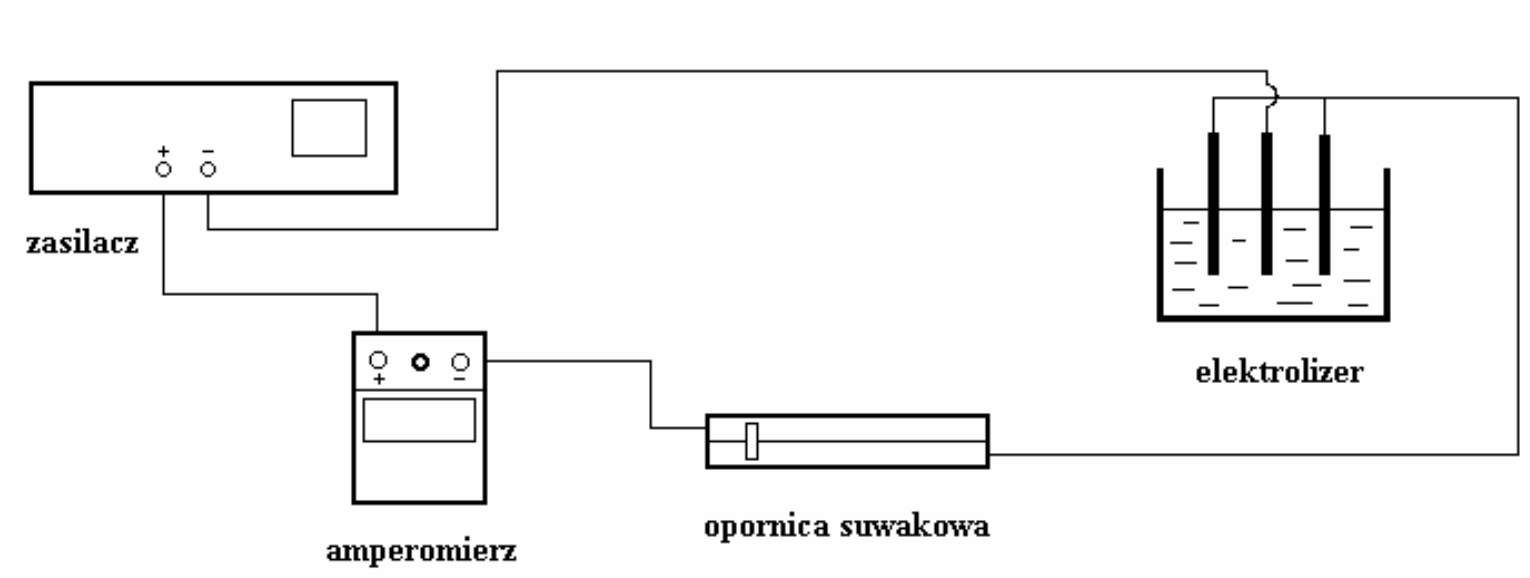
\includegraphics[width=0.6\textwidth]{uklad}
		\caption{Schemat zastosowanego obwodu elektrycznego}
		\label{fig:uklad}
	\end{figure}
	\begin{itemize}
		\item W pierwszym kroku, przy pomocy papieru ściernego, oczyszczono katodę i anody. Następnie zostały one przemyte bieżącą wodą i opłukane wodą destylowaną. Po czym, przy pomocy suszarki, dokładnie je wysuszono.
		
		\item W kolejnym kroku, po ostygnieciu elektrod, dokonano pomiaru ich mas.
		
		\item Następnie złożono układ zgodnie ze schematem(\ref{fig:uklad}). Po sprawdzeniu obwodu, uruchomiono zasilacz przy jednoczesnym rozpoczęciu pomiaru czasu.
		W czasie trwania elektrolizy dbano o utrzymanie stałego natężenia($0,5$ A).
		
		\item  Po upływie 30 minut wyłączono zasilanie i powtórnie zważono katodę i anody.
	\end{itemize}

	
	\section{Opracowanie danych pomiarowych}\label{sec:opr}
	\subsection{Pomiary i ich niepewności.}
	\begin{itemize}
		\item Masa
			
			\begin{table}
				\label{tab:masaPom}
				\caption{Pomiary mas}
				\begin{center}
				\begin{tabular}{p{0.1\linewidth}|p{0.13\linewidth}|p{0.15\linewidth}|p{0.1\linewidth}}
					&masa przed elektrolizą[g]&masa po elektrolizie[g]& różnica[g]\\
					\hline
					katoda&$75.448$&$75.744$&$0.296$ \\
					\hline
					anody &$201.460$&$201.170$&$0.290$ \\
				\end{tabular} 
					\end{center}	
			\end{table}
			

		Ze względu na zanieczyszczenia oraz ryzyko niedokładnego wysuszenia elektrod, przy pomiarach masy przyjęto niepewność większą od niepewności znamionowej użytej wagi($\Delta m=0.001$ g) równą $u(m)=0.003$. 
		
		\item Czas $ t=1800$s
		
		Niepewność zmierzonego czasu została pominięta ze względu na niezauważalny wpływ na wynik($\approx0.05$ \%). W dalszych obliczeniach nie uzwględniamy czasu 
		przy wyznaczaniu niepewności roszerzonych poszczególnych wielkości.
		
		\item Natężenie $I=0.5$A
		
		Niepewność natężenia wyznaczono ze wzoru:
	\end{itemize}
	\begin{equation}
	\label{eq:amper}
	u(I) = \frac{\text{klasa amperomierza} \cdot \text{zakres}}{100} = 3,75 \cdot 10^{-3} [A].
	\end{equation}

	\subsection{Wyznaczenie szukanych wielkości}
		Korzystając ze wzorów(\ref{eq:masa}), (\ref{eq:k}) i (\ref{eq:F}) oraz ze zmierzonych wielkości obliczono:
	\begin{itemize}
		
		\item elektrochemiczny równoważnik substancji $k$
		\begin{equation}
		k = \frac{m}{I t} = \frac{296 \cdot 10^{-3}}{0,5 \cdot 1,8 \cdot 10^3} \approx 3,288\cdot 10^{-4} \left[  \frac{g}{A \cdot s}\right] 
		\label{k_obliczone} 
		\end{equation}
		
		\item stała Faradaya $F$
		
		\begin{equation}
		F = \frac{\mu}{w k} = \frac{63,58 }{2 \cdot 3,219 \cdot 10^{-4}} \approx 96598  \left[  \frac{C}{mol}\right] 
		\label{F_obliczone} 
		\end{equation}
		
		\item ładunek elementarny $e$
		
		\begin{equation}
		e = \frac{F}{N_A} = \frac{96598 }{6,02 \cdot 10^{23}} \approx 1,604 \cdot 10^{-19}   \left[  C \right] 
		\label{e_obliczone} 
		\end{equation}
	\end{itemize}
 
 	
 	\subsection{Niepewności pomiarowe }
 	

 	Dla każdej z obliczonych wielkości wyznaczono niepewności pomiarowe. Do tego celu wykorzystano prawo przenoszenia dla niepewności względnej. Niepewność bezwględną wyznaczono jako iloraz niepewności względnej i obliczonej wartości.
 	Jak wspomniano wcześniej niepewność pomiaru czasu została pominięta.

 	\begin{equation}
 	\frac{u(k)}{k} = \sqrt{\left[\frac{u(m)}{m} \right]^2 + \left[\frac{u(I)}{I} \right]^2 } = \sqrt{\left[\frac{ 0,003}{0,296} \right]^2 + \left[\frac{0,00375}{0,5} \right]^2 } \approx 0,0126
 	\end{equation}
 	
 	\begin{equation}
 	u(k) = \frac{u(k)}{k} \cdot k =  0,0126 \cdot 0,3288 \cdot 10^{-3} \approx 0,0041 \cdot 10^{-3}  \left[  \frac{g}{A \cdot s}\right] 
 	\end{equation}
 	
	Dla stałej Faraday wyłącznie obliczona wartość równoważnika $k$ została obarczona błędem, dlatego jego złożona niepewność względna  jest równa niepewności względnej równoważnika $k$
 	\begin{equation}
 	\frac{u(F)}{F} = \sqrt{\left[\frac{u(\mu)}{\mu} \right]^2 + \left[\frac{u(k)}{k} \right]^2 } = \sqrt{\left[\frac{u(k)}{k} \right]^2 } = \frac{u(k)}{k}  ,
 	\end{equation}
 	
 	\begin{equation}
 	u(F) = F \frac{u(k)}{k}  =  96597  \cdot  0,0126 \approx 1217  \left[  \frac{C}{mol}\right] .
 	\end{equation}
 	
 	Analogicznie jak dla stałej Faradaya złożona niepewność względna ładunku równa jest tej wyznaczonej dla stałej Faradaya, a więc niepewności równoważnika $k$
 	\begin{equation}
 	\frac{u(e)}{e}=\sqrt{\left[\frac{u(F)}{F}\right]^2} =  \frac{u(F)}{F} =  \frac{u(k)}{k},
 	\end{equation}
 	
 	\begin{equation}
 	u(e) = e \frac{u(k)}{k}  =  1,604 \cdot 10^{-19}  \cdot  0,0126 \approx 0,0202 \cdot 10^{-19} [C] .
 	\end{equation}
 	
 	W celu sprawdzenia zgodności otrzymanych wyników z wartościami dokładnymi obliczono niepewność rozszerzoną jako $U(y)=2\cdot u(y)$.
	
	\section{Podsumowanie}
	\begin{table}[!h]
		\label{tab:pod}
		\caption{Podsumowanie wyników}
			\begin{tabular}{|p{0.08\linewidth}|c|c|c|c|c|}
			\hline  & wartość tablicowa($y_0$)  & wartość wyznaczona($y$)& $\frac{u(y)}{y}$ [\%] & $(y-U(y),y+U(y))$ & zgodność $y$ z $y_0$ \\ 
			\hline $k \left[  \frac{mg}{A \cdot s}\right]$ & 0,3294  & 0,3289  & 1,26  & (0,3247;0,333)  & Tak  \\ 
			\hline $F \left[  \frac{C}{mol}\right]$ & 96500 & 96597  & 1,26  & (95380;97815)  & Tak  \\ 
			\hline $e [10^{-19} C]$ & 1,6022   & 1,604    & 1,26    & (1,583;1,624)   & Tak  \\ 
			\hline 
		\end{tabular} 
	\end{table}

\vspace{1em}



\end{document}